\newcommand{\Titelpdf}{Thema2-Gr3-Kaur-Zeyse}
\newcommand{\DeinName}{Sumit Kaur und Simeon Zeyse}
\newcommand{\Matrikelnummer}{6059167 und 6056745}
\newcommand{\TitelArbeit}{Topic 2: Differentiability of colors in choropleth maps\\[0.4mm]}
\newcommand{\PrueferEins}{Prof. Dr.-Ing. Jochen Schiewe}
\newcommand{\artDerArbeit}{Seminar GIT}
\newcommand{\Datum}{\today}

%%%%%%%%%%%%%%%%%%%%%%%%%%%%%%%%%%%%%%%%%%%%%%%%%%%%%%%
%																					%
%	In dieser Datei werden alle Packages eingebunden, 	%
% welche f�r das Dokument n�tig sind. Desweiteren 		%
% werden die Dokumentinformationen gesetzt.						%
%																											%
%%%%%%%%%%%%%%%%%%%%%%%%%%%%%%%%%%%%%%%%%%%%%%%%%%%%%%%
%

%
\documentclass[pdftex, 		a4paper, 		% DIN A4 verwenden
							titlepage,	    % separate Titelseite
							%draft,			% Draft-Version, keine Bilder im pdf!
							emulatestandardclasses,
							final,			% Final-Version
							oneside,		% zweiseitiger Druck %X
							11pt,			% Schriftgr��e 12pt
							%BCOR20mm,		    			    %X
							DIV=calc,		
							headsepline,	
							%tocbasic,
							%openany,
							%pointlessnumbers
							]{article}	%	KOMAScript scrbook-Dokumentklasse							
%%%%%%%%%%%%%%%%%%%%%%%%%%%%%%%%%%%%%%%%%%%%%%%%%%%%%%%%
%	Einbinden der Pakete 
%%%%%%%%%%%%%%%%%%%%%%%%%%%%%%%%%%%%%%%%%%%%%%%%%%%%%%%%
\usepackage[a4paper, left=2.5cm, right=2.5cm, top=3cm, bottom=3cm, bindingoffset=0mm]{geometry}
%bindingoffset=15mm]
\usepackage[toc,page]{appendix}
\usepackage[ngerman,english]{babel}
\usepackage{multirow}
\usepackage{amsmath}
\usepackage{amssymb}
\usepackage[pdftex]{graphicx}
\usepackage{chngcntr}
\counterwithin{table}{section}
\counterwithin{figure}{section} %X
\counterwithin{equation}{section} %X
\usepackage{booktabs}
% PDF Dateien einbinden
\usepackage{pdfpages}
\usepackage{textcomp} 
\usepackage{upgreek}%kein Kursiv mehr
\pdfminorversion=6
\pdfcompresslevel=9

% Abstand zu Section...
%\RedeclareSectionCommand[beforeskip=-1.5\baselineskip,afterskip=.5\baselineskip]{section}
%\RedeclareSectionCommand[beforeskip=-.75\baselineskip,afterskip=.5\baselineskip]{subsection}
%\RedeclareSectionCommand[beforeskip=-.5\baselineskip,afterskip=.25\baselineskip]{subsubsection}
%\RedeclareSectionCommand[beforeskip=.5\baselineskip,afterskip=-1em]{paragraph}

\usepackage{textcomp} %griechische Alphabet nicht kursiv

%Einige Pakete haben Probleme mit dem Komaskript.
\usepackage{scrhack} 

\usepackage{xcolor}
\definecolor{urlLinkColor}{rgb}{0,0,0.5}
\definecolor{LinkColor}{rgb}{0,0,0}

\usepackage[center]{caption}

\usepackage{abstract} %Abstrakt

\usepackage{csquotes}
\usepackage[backend=biber,style= apa, sortcites = true]{biblatex}

\newcommand\ifintextcite{\ifdefstring{\blx@delimcontext}{textcite}} %parencite und textcite unterschiedlich
\DefineBibliographyStrings{german}{
	andothers = {\ifintextcite{and others}{et\addabbrvspace al.}},
%	nodate = {o.D.},
%	backrefpage  = {\lowercase :}
%	pages = {:}
}
\setlength{\bibitemsep}{12pt}
\addbibresource{source/bib/references.bib}
	
\usepackage[latin1]{inputenc} % Umlaute %  
\usepackage[scaled]{berasans}				% Schriftfamilie
\renewcommand{\rmdefault}{phv}
\renewcommand{\sfdefault}{phv}

% Grafikpaket
\usepackage{makeidx}   				% Paket zur Erzeugung eines Index
\usepackage[normalem]{ulem}   % bietet Unterstreichungsvarianten
%\usepackage{picins} 					% Bilder im Absatz platzieren
\usepackage[T1]{fontenc}			% Erweiterten Zeichensatz aktivieren
\usepackage{multido}					% erm�glicht Schleifenartiges wiederholen von Befehlen
\usepackage{mdwlist}					% erm�glicht das Setzen des Z�hlers bei Aufz�hlungspunkten
\usepackage{paralist}					% Paket f�r Aufz�hlungen, erweitert Enumerate-Paket
\usepackage{longtable}				% mehrseitige Tabellen
%\usepackage{tocloft}
\parindent0pt           			% verzichte auf Einr�cken der ersten Zeile
\parskip2ex            	% Abstand zwischen den Abs�tzen

\usepackage{floatflt,epsfig} %text neben Bild

%\usepackage{setspace}					% Paket zum Einstellen des Zeilenabstands
%\doublespacing								% doppelter Zeilenabstand
\linespread{1.5}


\usepackage{color}
\definecolor{hcu-blau}{RGB}{54, 141, 207}

% Farbeinstellungen f�r die Links im PDF Dokument.
%
\makeindex

%-----------Paket f�r absolute Positionierung von Grafiken------------------
\usepackage[absolute]{textpos}
\setlength{\TPHorizModule}{1mm}
\setlength{\TPVertModule}{\TPHorizModule}

%-----------Aufz�hlungen und Einstellungen f�r Sourcecode-------------------
%\usepackage[savemem]{listings} %Bei wenig Arbeitsspeicher dies Option [savemem] aktivieren.
\usepackage{listings}
\lstloadlanguages{TeX,XML, Java} % TeX sprache laden, notwendig wegen option 'savemem'
\lstset{%
	language=[LaTeX]TeX,     % Sprache des Quellcodes ist TeX
	numbers=left,            % Zelennummern links
	stepnumber=1,            % Jede Zeile nummerieren.
	numbersep=5pt,           % 5pt Abstand zum Quellcode
	numberstyle=\tiny,       % Zeichengr�sse 'tiny' f�r die Nummern.
	breaklines=true,         % Zeilen umbrechen wenn notwendig.
	breakautoindent=true,    % Nach dem Zeilenumbruch Zeile einr�cken.
	postbreak=\space,        % Bei Leerzeichen umbrechen.
	tabsize=2,               % Tabulatorgr�sse 2
	basicstyle=\ttfamily\footnotesize, % Nichtproportionale Schrift, klein f�r den Quellcode
	showspaces=false,        % Leerzeichen nicht anzeigen.
	showstringspaces=false,  % Leerzeichen auch in Strings ('') nicht anzeigen.
	extendedchars=true,      % Alle Zeichen vom Latin1 Zeichensatz anzeigen.
	backgroundcolor=\color{ListingBackground}} % Hintergrundfarbe des Quellcodes setzen.


\lstset{
  basicstyle=\small\ttfamily,
  columns=fullflexible,
  showstringspaces=false,
  %commentstyle=\color{gray}\upshape
}
%neue Lang definieren, als Bsp.
\lstdefinelanguage{XML-changed}
{
  basicstyle=\footnotesize\ttfamily\bfseries,
  morestring=[b]",
  morestring=[s]{>}{<},
  morecomment=[s]{<?}{?>},
  stringstyle=\color{black},
  identifierstyle=\color{darkblue},
  keywordstyle=\color{cyan},
  morekeywords={xmlns,version,type}% list your attributes here
}

%-----------Caption Package-------------------
\usepackage{caption}
\usepackage{subcaption}
\DeclareCaptionFont{hcu-blau}{\color{hcu-blau}}

\usepackage{silence}
\WarningFilter{scrbook}{Usage of package `fancyhdr'}

\usepackage[labelfont = {bf,it}, font={footnotesize,it}, labelsep = space]{caption} %Beschirftung Tabelle/Abbildung

%\usepackage[labelfont={hcu-blau,{bf}}]{caption}
\renewcommand{\arraystretch}{1.0}   %tabellenabstand

\usepackage[labelfont = {bf,it}, font={footnotesize,it}, labelsep = space]{subcaption}

%-----------Header+Footer---------------------------------------------------
%\usepackage{fancyhdr}					
%\pagestyle{fancy}
%\fancyhf{}							
%\lhead{\leftmark}
%\rhead{\DeinName}
%\rfoot{\thepage} 
%\fancyfoot[EL]{\thepage}   %Seitenzahl abwechselt
%\fancyfoot[OR]{\thepage}   %Seitenzahl abwechselt
%\renewcommand{\headrulewidth}{0.2pt} % Kopflinie
%\renewcommand{\sectionmark}[1]{\markleft{\arabic{chapter}.\arabic{section}\ #1}}

%--------------------------------------------------------------------------------

\usepackage{scrlayer-scrpage}
\pagestyle{scrheadings}
\clearpairofpagestyles

\ohead{\pagemark}
%\chead{Kopfzeile Mitte}
\ihead{\leftmark}
%\ifoot{Fu�zeile innen}
%\cfoot{Fu�zeile Mitte}
%\ofoot{\pagemark}

%\renewcommand*\chapterpagestyle{scrheadings}
\renewcommand{\sectionmark}[1]{\markleft{\arabic{section}\ #1}}
%--------------------------------------------------------------------------------

% -------F�r ToDo-Notes--------------------------------------------------------------------
\usepackage[color=red, shadow]{todonotes} % ", disable" deaktiviert ToDo-Notes
%Vereinfachtes "Inline-Todo"
\newcommand{\td}[1]{{\todo[inline]{#1}}}
\newcommand{\tdu}[1]{{\todo[inline, color=green!40]{#1}}}

%--------F�r Links-------------------------------------------------------------------------
%--------HyperRef konfigurieren-------------------------------------------------------------------------

\usepackage[
	pdftitle={\Titelpdf},
	pdfauthor={\DeinName},
	pdfsubject={\TitelArbeit},
	pdfcreator={MiKTeX, LaTeX with hyperref and KOMA-Script auf Basis der Vorlage von seiler.it},
	pdfkeywords={Bachelorarbeit, Hamburg, HafenCity Universit�t},%weitere Keywords hier einf�gen
	pdfpagemode=UseOutlines,%                                  
	pdfdisplaydoctitle=true,%                                  
	pdflang=de%                                              
]{hyperref}

\hypersetup{%
	colorlinks=true,%        Aktivieren von farbigen Links im Dokument (keine Rahmen)
	linkcolor=LinkColor,%    Farbe festlegen.
	citecolor=LinkColor,%    Farbe festlegen.
	filecolor=LinkColor,%    Farbe festlegen.
	menucolor=LinkColor,%    Farbe festlegen.
	urlcolor=LinkColor,%     Farbe von URL's im Dokument.
	bookmarksnumbered=true%  �berschriftsnummerierung im PDF Inhalt anzeigen.
}


% Beginn des Dokuments
\begin{document}
%\nocite{*}

\begin{titlepage}

\newgeometry{left=2cm, right=2cm, top=2cm, bottom=2cm}	
\begin{center}
	
\begin{figure}
\centering

\includegraphics[width=0.2\linewidth]{source/images/hcu_logo}	
\end{figure}

{\normalsize HafenCity University Hamburg}\\[1mm]
{\normalsize University Of The Built Environment And Metropolitan Development}\\[8mm] 
\textbf{\large{\artDerArbeit}}\\[20mm]

\textbf{\LARGE \TitelArbeit}\vspace{3cm}

\vspace{0.2cm}

{\normalsize Study program:}\\[.8mm]
\textbf{{\large Geodesy and Geoinformatics}\\[3mm]}

\vspace{0.2cm}

{\normalsize Matriculation number:}\\[.8mm]
\textbf{{\large \Matrikelnummer}\\[3mm]}

\vspace{0.2cm}

{\normalsize Professor:}\\[.8mm]
\textbf{{\large \PrueferEins}}

\vspace{0.2cm}

{\normalsize Group 3:}\\[.8mm]
\textbf{\large \DeinName}\\
\bigskip
\bigskip
\bigskip
\bigskip

\Datum
\end{center}
\end{titlepage}
%\frontmatter
\pagenumbering{Roman} 
\tableofcontents
\clearpage
\listoffigures
\listoftables
\clearpage
\pagenumbering{arabic}
%\mainmatter
% Abstand Gleichung und Text
\setlength\abovedisplayskip{8pt}
\setlength\belowdisplayskip{8pt}
\section{Hypothese}
Die Differenzierbarkeit von Farben beim Betrachten von Choroplethenkarten h�ngt vorallem von der Farbdistanz zwischen den Farben und der Anzahl der Farbklassen ab.

\section{Introduction}
From a designer's perspective, colors play an essential role in cartography. Nevertheless, according to \textcite{brychtovaC2017}, there is little research to empirically determine the minimum effective color distance to safely and correctly distinguish cartographic symbols. 

The ability to distinguish colors and shades of the same color plays an important role in cartography \parencite{coltekin2017}.

Even subtle manipulation of color spacing shows significant effects on the impact on overall readability of a map \parencite{brychtovaC2015, brychtovaV2014}. 

Lack of proper visual distance in variables colour hue and colour value is a known contributor to legibility problems in map use tasks \parencite{chesneau2007, steinrucken2013, stigmar2010}.

\subsection{Simple Choropleth maps}
Unlike chorochromatic maps, which visualize nominal (qualitative) data, simple choropleth maps have made it their business to display quantitative data in terms of area. In doing so, hue, saturation and brightness are used to show corresponding changes in the data. Although in theory choropleth maps are only useful for data related to areas (Bollmann et al. 2001), in practice they are also used for non-area related data. E.G. \textcolor{red}{???} \parencite{hruby2016, schiewe2015}.

Some advantages of choropleth maps are e.g. the simplified visibility. For this, the data are classified. For example, one can distinguish between an equal interval and a quantile class division. With equal interval each class possesses the same size independently of its occupation, whereas with a quantile class division each class contains the same number of elements. Depending on the use case and data frequency, one or the other class division is more suitable, because they have a significant influence on the appearance of a map \parencite{schiewe2015, rahlf2020}.

Due to the public availability of static data, the production of these maps is easy and can be linked, analyzed, classified and visualized with any suitable GIS software \parencite{hruby2016}.

\section{Basic color information}

\subsection{Human' color perception}
Although our current understanding is that color vision results from the response of three photoreceptor cells in the retina to incident light, their perception cannot be fully understood. This may be due to both individual and environmental factors that influence color perception \parencite{lafer2015, xiao2016}.

Some of these factors can be, for example, the amount of light in the environment, shadows, surrounding materials, and reflectivity. In addition, the viewer's prior knowledge and cognitive biases play a significant role in color perception \parencite{derefeldt2004, foster2011}.

In addition, there is evidence that the number and distribution of photoreceptors in the eye influences what we see \parencite{roy1991}, and that our brain assumes a particular direction or light source e.g., \parencite{gegenfurtner2015, lafer2015}.

Thus, it can be said that the color perception of an individual is not stable over space and time. The same is true not only for individuals but also for groups.  

Nevertheless, there are many efforts to model and quantify color perception such as mathematical models that attempt to determine thresholds by which two colors or shades of the same color become distinguishable. 

This color distance describes a metric that quantifies the human ability to visually distinguish differences between two colors see chapter \ref{subsection:distance} \parencite{coltekin2017}.

\subsection{Color spaces}
There are a lot of color models that have set themselves the task of representing the logic of generating colors \parencite{kuehni2001}. These color models can be divided into four main groups: instrumental, pseudo-perceptual, colorimetric, and perceptual unitary color models.

Instrumental color models include, for example, RBG or CMYK. Pseudoperceptual color models are e.g. HVS or HSB, whereas colorimetric color models are represented e.g. by CIE 1931 XYZ. To the latter model (perceptually uniform) belong for example the Munsell system, CIELAB or CIELUV. The most frequently used color models are the CIE 1931 XYZ or CIELAB. 

A color space is understood to be all existing colors that can be represented e.g. by a screen, printer or the human eye, which are generated from a combination of the components of a model \parencite{munsell1915}.

\section{Criteria}

\subsection{Color distance}\label{subsection:distance}
Visual distance in cartography is understood as a measurement of differences between visual variables such as size, shape and orientation \parencite{brychtova2015}. Here we focus on the variable of color hue and color value. The human perceived difference between two colors or color shades can be described as the color distance. In other words, certain change of colour in the perceptually uniform space produces equal change in human perception of that colour \parencite{brychtovaC2017}.

To describe the distance of two colors scientistis have developed a method to describe the color distance. To express color quantitatively a colour space corresponding to the human perception is needed. Such color spaces are called perceptually uniform or linear. The use of such color spaces try to ensure results of color distance which are proportional to the human perception \parencite{brychtova2015}. Presently the CIEDE2000 model ($\Delta E_{00}$, equation defined in \textcite{brychtova2015}) is regarded as the best coinciding color distance model with visual perception. 
 
The colors of digital maps are usually represented in the RGB color space, since the colors on most, if not all, digital screens are generated with these three colors (red, green, blue). However RGB values do not lead to specific color if they are not related to an absolut color space such as sRGB, Adobe RGB or ProPhoto RGB. To use the most realistic color space, colors should be specified and selected in the sRGB color space in the initial situation. Why most realistic? As mentioned before sRGB is the smallest color space of the three. The vast majority of digital screens cannot create all Adobe RGB or even ProPhoto RGB colors. Even sRGB isn't fully supported by cheap laptop screens. However sRGB is known as the default color space \parencite{kenrockwell2006}. Therefore sRGB should be choosed to increase the chance that the users screen actually is able to display the color which was choosed by the creater of a map. 

\subsubsection{Equation}\label{subsec:equation}
The first step to calculate the color distance $\Delta E_{00}$ is the transformation from the original color space (as mentioned above this would be sRGB in most cases) to the CIE 1931 XYZ color space. For that the RGB values have to be normalized so the values lie in the interval [0; 1]. 

\begin{equation}
R_{lin} = G_{lin} = B_{lin} =
	\begin{cases}
		\frac{V_{R,G,B}}{12.92}, & \text{if $V_{R,G,B} \leq 0.04045$}\\
		\sqrt[5]{(\frac{R + 0.055}{1 + 0.055})^{12}}, & \text{otherwise}
	\end{cases}
\end{equation}
\begin{equation}
\left[ \begin{array}{r}
X \\ 
Y \\
Z \\ 
\end{array}\right] = \left[ \begin{array}{rrr}
0.4124 & 0.3576 & 0.1805 \\ 
0.2126 & 0.7152 & 0.0722 \\
0.0193 & 0.1192 & 0.9505 \\ 
\end{array}\right] \left[ \begin{array}{r}
R_{lin} \\ 
G_{lin} \\
B_{lin} \\ 
\end{array}\right]
\end{equation}

The second step is the transformation of the colors into CIE Lab. The CIELAB Colorspace, also known as CIE 1976 (L*, a*, b*) describes all colors perceptible by human eyes \parencite{levkowitz1997}. It consists of three components: L describes the brightness [0 - 100], a describes the axis between red and green and b describes the axis of the blue and yellow colors. While negative values stand for green/blue colors and positive values for magenta and yellow). Theoretically the a and b values are not limited but in praxis human eyes can only see colors upin a specific value. 

\begin{equation}
L = 116 f\left(\frac{Y}{Y_{n}}\right)-16
\end{equation}
\begin{equation}
a = 500 \left[f\left(\frac{X}{X_{n}}\right)-f\left(\frac{Y}{Y_n}\right)\right]
\end{equation}
\begin{equation}
b = 200 \left[f\left(\frac{Y}{Y_{n}}\right)-f\left(\frac{Z}{Z_n}\right)\right]
\end{equation}
where
\begin{equation}
f(t) =
\begin{cases}
	\sqrt[3]{t}, & \text{if $t > (\frac{6}{29})^{3}$}\\
	\frac{1}{3}(\frac{29}{6})^{3}t+\frac{4}{29}, & \text{otherwise}
\end{cases}
\end{equation}

Finally the last step is to calculate the color distance $\Delta E_{00}$ between two colors with the CIEDE2000 model. However the following equation takes three parametric coefficents $k_{L}, k_{C}$ and $k_{H}$ to adjust the equation according to observer enviroment.

\begin{equation}
\Delta E_{00}= \sqrt{\left(\frac{\Delta L'}{k_{L}S_{L}}\right)^{2}+\left(\frac{\Delta C'}{k_{C}S_{C}}\right)^{2}+\left(\frac{\Delta H'}{k_{H}S_{H}}\right)^{2}+R_{T}\frac{\Delta C'}{k_{C}S_{C}}\frac{\Delta H'}{k_{H}S_{H}}}
\end{equation}

where $\Delta L'$, $\Delta C'$ and $\Delta H'$ are the CIELAB metric lightness, chroma, and hue differences, calculated
between the standard and sample in a pair and $S_{L}$, $S_{C}$ and $S_{H}$ are the weighting functions for the lightness,
chroma, and hue components.  However, since the formulas are quite extensive, the equations can be read in the appendix \ref{further equation}.
The $k_{L}$, $k_{C}$ and $k_{H}$ values are the parametric factors to be adjusted according to different viewing parameters such as textures, backgrounds, separations etc. \parencite{luo2001}.

\subsection{Number of classes}

Obviously the number of classes also has an impact on the differentiability of colors. For example if we reduce the number of classes to 1 (which makes no sense in practice) the color will be determined in hopefully all cases. The more classes we create, the harder it becomes to tell the colors apart as the propability decreases. In addition to that it is clear that the color distance decreases with more classes as the number of color shades are limited by the color space. 

\textcite{brychtovaC2017} makes the finding that with ColorBrewer 2.0 the color distance becomes smaller the more classes are used, which is to be expected. For the selected 18 sequential schemes, the color distance was analyzed and calculated between 3, 6 and 9 classes. These numbers of classes were selected according to \textcite{brychtovaC2017}, since they represent the minimum, maximum and middle of the class selection. Thus, the results (see table \ref{tab:classes}) show that the number of classes have an influence on how the distance of the colors is chosen and thus becomes distinguishable to the human eye. 

\begin{table}[h!]
\centering
\caption[Color distance depending on number of classes]{Color distance depending on number of classes \\ (According to \textcite{brychtovaC2017})}
	\begin{tabular}{c c c c }
		\hline
		\hline
		Number of classes & $\Delta E_{00}min$ & $\Delta E_{00}max$ & $\Delta E_{00}mean$ \\ 
		\hline
		\hline
		3 & 11.26 & 33.92 & 20.61 \\  
		6 & 6.24 & 26.44 & 12.41 \\
		9 & 3.04 & 20.46 & 10.28   
	\end{tabular}
\label{tab:classes}
\end{table}

\subsection{Further aspects}

\subsubsection{Spatial distance}
The greater the spatial distance between two color cells, the more the ability to distinguish the colors decreases. This is true for both sequential and qualitative schemes. However, at a color distance of $\Delta E_{00}$ = 10, the accuracy of color discrimination increases, even at relatively large spatial distances \parencite{brychtovaC2017}. 

\subsubsection{Brightness of colors}

An evaluting case study of color distances in ColorBrewer 2.0 from \textcite{brychtovaC2017} has investigated the color distances in 18 color schemes made by colorBrewer 2.0. All color chemes were investigated with 9, 6 and 3 classes. As a result \textcite{brychtovaC2017} figured out that mostly the darker the color becomes, the larger the color distance becomes. Therefore it can be assumed that the deveolpers of ColorBrewer 2.0 came to the result that darker colors needs a larger color distance to correctly determine a difference between colors. Color schemes with 9 classes show their largest color distances in the darker middle colors.

Bild einf�gen. 

\section{Examples}
\subsection{ColorBrewer2.0}
Brewer and her colleagues \parencite{brewer2003, brewer1994, brewer1996, brewer1997, brewer1999} did research on color, developing color schemes to viualize both quantitative and qualitative data. In the process, the online software ColorBrewer 2.0 was developed, which can be very helpful for many applications. ColorBrewer 2.0 offers the user a choice between 18 sequential, 9 divergent and 8 qualitative color schemes. Depending on the selection, a distinction can be made between 3 and 12 classes. They used Munsell diagrams to design color schemes that would maintain consistency in perceived color distances between classes \parencite{brychtovaC2017}. 

The Munsell Color System is a color system that is the first complete, most widely used, and still in use today. It is based on three essential criteria: Hue, Chroma and Value, with Hue being the most important criterion (\ref{fig:munsell}). Munsell chose five main hues: red (R), yellow (Y), green (G), blue (B) and purple (P). Now he subdivides the perceptible color nuances into further color tones, which are to represent the intermediate color tones: YR (yellow-red), GY (green-yellow), BG (blue-green), PB (purple-blue) and RP (red-purple). These ten hues are further subdivided a few times into ten gradations. Numbers from 0 to 10 are also added to the hues. Towards the outside, the saturation of the color (chroma) increases. The vertical center axis, which ranges from white (value 10) to black (value 0), which can be represented with colorants, is represented by the value. This results in a 10-row gray scale \parencite{munsell1915}.

\begin{figure}
	\centering
	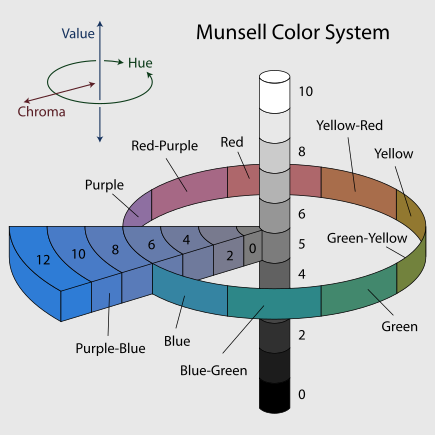
\includegraphics[width=0.4\linewidth]{source/images/munsell}
	\caption{Munsell Color System \\
	(Source: \textcite{munsell2007})}
	\label{fig:munsell}
\end{figure}

\subsection{Sequential color scheme generator}
To develop a suitable sequential color scheme, the analytical geometry is calculated. The intersection of two subspaces is searched for. This is the intersection of the CIELAB color space and a straight line on which the color scheme lies.

For this we look which color tones lie on the straight line. This follows at given distances defined with CIEDE2000. 

It must be kept in mind that this method is only suitable for the creation of schemata that are to be used for digital maps. Therefore its construction is limited by the sRGB color space. 

This method shows a reverse approach to design color schemes based on the color distance as described in chapter \ref{subsec:equation} \parencite{brychtovaC2017}. The online tool Color Scheme Generator 1.0 has implemented this software (freely available at: http://eyetracking.upol.cz/color).

The user of this online tool can display a color scheme by selecting a base color of the whole scheme, the color classes and the CIEDE2000 color distances between the classes \parencite{brychtovaDole2015}

\section{Conclusion}


Colors which can not be differentiated correctly and quickly are a main problem when reading choropletic maps. it can lead to errors when it comes to understanding and interpretating the map. Therefore the selection of colors should be done wisely.

The percptation of colors by human eyes is not stable, it is affected by enviroment light, shadows and sorrounding materials. In addition the color perceptation differs from human to human and also changes with time. Extrem examples of course are colorblind people. 

Irgendwas �ber color spaces.

It can be concluded, that the ability to differentiate colors on a choropletic map is mainly affected by the color distance. The color distance is a measure to quantify the difference of two colors or shades of a color from the perspective of an human eye. 
Another aspect which is closly connected to the color distance is the number of classes. Since the colors are limited by the color space sRGB the color distances is likely to become smaller when choosing more classes. 
In addition to that the spatial distance between two colors also has an impact how precisly humans can differ the colors.
\textcite{brychtovaC2017} has figured out that the color schmes at the well known software ColorBrewer 2.0 tend to have wider colors distances at dark colors, which is an indicator that darker colors are more difficult to differentiate. A thesis which could be evaluated further also with the ulterior motive that the calculation of the color distance does consider the brightness of the color.

Examples for usefull software when selection color schemes and specific colors for chorpletic maps are ColorBrewer 2.0 and Sequential Color Scheme Generator. Last one is definatly a tool for map creators with previous knowledge about color distance. 

Der Farbabstand (eine von der International Commission on Illumination zur Quantifizierung der menschlichen F�higkeit, zwischen Farben zu unterscheiden) wurde empirisch nachgewiesen, dass er ein wichtiger Faktor f�r die Lesbarkeit von Karten insgesamt ist (z. B. Brychtova und Coltekin 2015, Brychtova 2015, Brychtova und Coltekin 2014, Brychtova und Vondrakova 2014). Unzureichender Farbabstand zwischen kartografischen Symbolen beeintr�chtigt die F�higkeit der Kartennutzer, die und Interpretation der visualisierten r�umlichen Informationen.\parencite{brychtovaDole2015}



%\bibliography
\appendix
\section{Further equation}\label{further equation}
\begin{equation}
C_{1,ab}=\sqrt{(a_{1})^{2}+(b_{1})^{2}} \quad C_{2,ab}=\sqrt{(a_{2})^{2}+(b_{2})^{2}}
\end{equation}
\begin{equation}
\bar{C}_{ab}=\frac{C_{1,ab}+C_{2,ab}}{2}
\end{equation}
\begin{equation}
G = 0.5(1-\sqrt{\frac{\bar{C}_{ab}^{7}}{\bar{C}_{ab}^{7}+25^7}})
\end{equation}
\begin{equation}
a_{1}'=(1+G)a_{1} \quad a_{2}'=(1+G)a_{2} 
\end{equation}
\begin{equation}
C_{1}'=\sqrt{(a_{1}')^{2}+(b_{1})2} \quad C_{2}'=\sqrt{(a_{2}')^{2}+(b_{2})2}
\end{equation}
\begin{equation}
h_{1}' = atan2(b_{1},a_{1}') =
\begin{cases}
tan^{-1}(\frac{b_{1}}{a_{1}'}) & b_{1}>0,a_{1}' \geq 0\\
tan^{-1}(\frac{b_{1}}{a_{1}'})+180^{\circ} & b_{1}<0\\
tan^{-1}(\frac{b_{1}}{a_{1}'})+360^{\circ} & b_{1}>0,a_{1}'<0 \\
90^{\circ} & b_{1}=0,a_{1}'>0\\
270^{\circ} & b_{1}=0,a_{1}'<0\\
0^{\circ} & b_{1}=0,a_{1}'=0
\end{cases}
\end{equation}
\begin{equation}
h_{2}' = atan2(b_{2},a_{2}') =
\begin{cases}
tan^{-1}(\frac{b_{2}}{a_{2}'}) & b_{2}>0,a_{2}' \geq 0\\
tan^{-1}(\frac{b_{2}}{a_{2}'})+180^{\circ} & b_{2}<0\\
tan^{-1}(\frac{b_{2}}{a_{2}'})+360^{\circ} & b_{2}>0,a_{2}'<0 \\
90^{\circ} & b_{2}=0,a_{2}'>0\\
270^{\circ} & b_{2}=0,a_{2}'<0\\
0^{\circ} & b_{2}=0,a_{2}'=0
\end{cases}
\end{equation}
\begin{equation}
\Delta L'=L_{2}-L_{1}
\end{equation}
\begin{equation}
\Delta C'=C_{2}'-C_{1}'
\end{equation}
\begin{equation}
\Delta h' =
\begin{cases}
0 & C_{1}'C_{2}'=0\\
h_{2}'-h_{1}' & C_{1}'C_{2}'\ne q0, |h_{2}'-h_{1}'| \geq -180^{\circ}\\
(h_{2}'-h_{1}')-360^{\circ} & C_{1}'C_{2}'\neq 0, (h_{2}'-h_{1}') > -180^{\circ}\\
(h_{2}'-h_{1}')+360^{\circ} & C_{1}'C_{2}'\neq 0, (h_{2}'-h_{1}') < -180^{\circ}
\end{cases}
\end{equation}
\begin{equation}
\Delta H'=2\sqrt{C_{1}'C_{2}'}sin(\frac{\Delta h'}{2})
\end{equation}
\begin{equation}
\bar{L}'=\frac{L_{1}+L_{2}}{2}
\end{equation}
\begin{equation}
\bar{C}'=\frac{C_{1}'+C_{2}'}{2}
\end{equation}
\begin{equation}
\bar{h'} =
\begin{cases}
\frac{h_{1}'+h_{2}'}{2} & C_{1}'C_{2}'\neq 0 \wedge |h_{2}'-h_{1}'| \leq 180^{\circ}\\
\frac{h_{1}'+h_{2}'+360^{\circ}}{2}& |h_{2}'-h_{1}'| > 180^{\circ} \wedge (h_{2}'-h_{1}') < 180^{\circ}\\
\frac{h_{1}'+h_{2}'-360^{\circ}}{2} & |h_{2}'-h_{1}'| > 180^{\circ} \wedge (h_{2}'-h_{1}') \geq 360^{\circ}\\
h_{1}'+h_{2}' & C_{1}'C_{2}'=0
\end{cases}
\end{equation}
\begin{equation}
T=1-0.17 cos(\bar{h}'-30^{\circ})+0.24 cos(2\bar{h}')+0.32(3\bar{h}'+6^{\circ})-0.2 cos(4\bar{h}'-63^{\circ})
\end{equation}
\begin{equation}
\Delta 0 = 30e^{-(\frac{h'-275^{\circ}}{25})^{2}}
\end{equation}
\begin{equation}
R_{c}=2\sqrt{\frac{\bar{C'}_{ab}^{7}}{\bar{C'}_{ab}^{7}+25^{7}}}
\end{equation}
\begin{equation}
S_{L}=1+\frac{0.015(\bar{L}'-50)^{2}}{\sqrt{20+(\bar{L}'-50)^{2}}}
\end{equation}
\begin{equation}
S_{C}=1+0.0045\bar{C}'
\end{equation}
\begin{equation}
S_{H}=1+0.0045\bar{C}'T
\end{equation}
\begin{equation}
R_{T}=-sin(2 \Delta 0)R_{c}
\end{equation}
%\addcontentsline{toc}{section}{Bibliography}
%\backmatter
\printbibliography[title = Bibliography]
\end{document}


